
% Default to the notebook output style

    


% Inherit from the specified cell style.




    
\documentclass[11pt]{article}

    
    
    \usepackage[T1]{fontenc}
    % Nicer default font (+ math font) than Computer Modern for most use cases
    \usepackage{mathpazo}

    % Basic figure setup, for now with no caption control since it's done
    % automatically by Pandoc (which extracts ![](path) syntax from Markdown).
    \usepackage{graphicx}
    % We will generate all images so they have a width \maxwidth. This means
    % that they will get their normal width if they fit onto the page, but
    % are scaled down if they would overflow the margins.
    \makeatletter
    \def\maxwidth{\ifdim\Gin@nat@width>\linewidth\linewidth
    \else\Gin@nat@width\fi}
    \makeatother
    \let\Oldincludegraphics\includegraphics
    % Set max figure width to be 80% of text width, for now hardcoded.
    \renewcommand{\includegraphics}[1]{\Oldincludegraphics[width=.8\maxwidth]{#1}}
    % Ensure that by default, figures have no caption (until we provide a
    % proper Figure object with a Caption API and a way to capture that
    % in the conversion process - todo).
    \usepackage{caption}
    \DeclareCaptionLabelFormat{nolabel}{}
    \captionsetup{labelformat=nolabel}

    \usepackage{adjustbox} % Used to constrain images to a maximum size 
    \usepackage{xcolor} % Allow colors to be defined
    \usepackage{enumerate} % Needed for markdown enumerations to work
    \usepackage{geometry} % Used to adjust the document margins
    \usepackage{amsmath} % Equations
    \usepackage{amssymb} % Equations
    \usepackage{textcomp} % defines textquotesingle
    % Hack from http://tex.stackexchange.com/a/47451/13684:
    \AtBeginDocument{%
        \def\PYZsq{\textquotesingle}% Upright quotes in Pygmentized code
    }
    \usepackage{upquote} % Upright quotes for verbatim code
    \usepackage{eurosym} % defines \euro
    \usepackage[mathletters]{ucs} % Extended unicode (utf-8) support
    \usepackage[utf8x]{inputenc} % Allow utf-8 characters in the tex document
    \usepackage{fancyvrb} % verbatim replacement that allows latex
    \usepackage{grffile} % extends the file name processing of package graphics 
                         % to support a larger range 
    % The hyperref package gives us a pdf with properly built
    % internal navigation ('pdf bookmarks' for the table of contents,
    % internal cross-reference links, web links for URLs, etc.)
    \usepackage{hyperref}
    \usepackage{longtable} % longtable support required by pandoc >1.10
    \usepackage{booktabs}  % table support for pandoc > 1.12.2
    \usepackage[inline]{enumitem} % IRkernel/repr support (it uses the enumerate* environment)
    \usepackage[normalem]{ulem} % ulem is needed to support strikethroughs (\sout)
                                % normalem makes italics be italics, not underlines
    

    
    
    % Colors for the hyperref package
    \definecolor{urlcolor}{rgb}{0,.145,.698}
    \definecolor{linkcolor}{rgb}{.71,0.21,0.01}
    \definecolor{citecolor}{rgb}{.12,.54,.11}

    % ANSI colors
    \definecolor{ansi-black}{HTML}{3E424D}
    \definecolor{ansi-black-intense}{HTML}{282C36}
    \definecolor{ansi-red}{HTML}{E75C58}
    \definecolor{ansi-red-intense}{HTML}{B22B31}
    \definecolor{ansi-green}{HTML}{00A250}
    \definecolor{ansi-green-intense}{HTML}{007427}
    \definecolor{ansi-yellow}{HTML}{DDB62B}
    \definecolor{ansi-yellow-intense}{HTML}{B27D12}
    \definecolor{ansi-blue}{HTML}{208FFB}
    \definecolor{ansi-blue-intense}{HTML}{0065CA}
    \definecolor{ansi-magenta}{HTML}{D160C4}
    \definecolor{ansi-magenta-intense}{HTML}{A03196}
    \definecolor{ansi-cyan}{HTML}{60C6C8}
    \definecolor{ansi-cyan-intense}{HTML}{258F8F}
    \definecolor{ansi-white}{HTML}{C5C1B4}
    \definecolor{ansi-white-intense}{HTML}{A1A6B2}

    % commands and environments needed by pandoc snippets
    % extracted from the output of `pandoc -s`
    \providecommand{\tightlist}{%
      \setlength{\itemsep}{0pt}\setlength{\parskip}{0pt}}
    \DefineVerbatimEnvironment{Highlighting}{Verbatim}{commandchars=\\\{\}}
    % Add ',fontsize=\small' for more characters per line
    \newenvironment{Shaded}{}{}
    \newcommand{\KeywordTok}[1]{\textcolor[rgb]{0.00,0.44,0.13}{\textbf{{#1}}}}
    \newcommand{\DataTypeTok}[1]{\textcolor[rgb]{0.56,0.13,0.00}{{#1}}}
    \newcommand{\DecValTok}[1]{\textcolor[rgb]{0.25,0.63,0.44}{{#1}}}
    \newcommand{\BaseNTok}[1]{\textcolor[rgb]{0.25,0.63,0.44}{{#1}}}
    \newcommand{\FloatTok}[1]{\textcolor[rgb]{0.25,0.63,0.44}{{#1}}}
    \newcommand{\CharTok}[1]{\textcolor[rgb]{0.25,0.44,0.63}{{#1}}}
    \newcommand{\StringTok}[1]{\textcolor[rgb]{0.25,0.44,0.63}{{#1}}}
    \newcommand{\CommentTok}[1]{\textcolor[rgb]{0.38,0.63,0.69}{\textit{{#1}}}}
    \newcommand{\OtherTok}[1]{\textcolor[rgb]{0.00,0.44,0.13}{{#1}}}
    \newcommand{\AlertTok}[1]{\textcolor[rgb]{1.00,0.00,0.00}{\textbf{{#1}}}}
    \newcommand{\FunctionTok}[1]{\textcolor[rgb]{0.02,0.16,0.49}{{#1}}}
    \newcommand{\RegionMarkerTok}[1]{{#1}}
    \newcommand{\ErrorTok}[1]{\textcolor[rgb]{1.00,0.00,0.00}{\textbf{{#1}}}}
    \newcommand{\NormalTok}[1]{{#1}}
    
    % Additional commands for more recent versions of Pandoc
    \newcommand{\ConstantTok}[1]{\textcolor[rgb]{0.53,0.00,0.00}{{#1}}}
    \newcommand{\SpecialCharTok}[1]{\textcolor[rgb]{0.25,0.44,0.63}{{#1}}}
    \newcommand{\VerbatimStringTok}[1]{\textcolor[rgb]{0.25,0.44,0.63}{{#1}}}
    \newcommand{\SpecialStringTok}[1]{\textcolor[rgb]{0.73,0.40,0.53}{{#1}}}
    \newcommand{\ImportTok}[1]{{#1}}
    \newcommand{\DocumentationTok}[1]{\textcolor[rgb]{0.73,0.13,0.13}{\textit{{#1}}}}
    \newcommand{\AnnotationTok}[1]{\textcolor[rgb]{0.38,0.63,0.69}{\textbf{\textit{{#1}}}}}
    \newcommand{\CommentVarTok}[1]{\textcolor[rgb]{0.38,0.63,0.69}{\textbf{\textit{{#1}}}}}
    \newcommand{\VariableTok}[1]{\textcolor[rgb]{0.10,0.09,0.49}{{#1}}}
    \newcommand{\ControlFlowTok}[1]{\textcolor[rgb]{0.00,0.44,0.13}{\textbf{{#1}}}}
    \newcommand{\OperatorTok}[1]{\textcolor[rgb]{0.40,0.40,0.40}{{#1}}}
    \newcommand{\BuiltInTok}[1]{{#1}}
    \newcommand{\ExtensionTok}[1]{{#1}}
    \newcommand{\PreprocessorTok}[1]{\textcolor[rgb]{0.74,0.48,0.00}{{#1}}}
    \newcommand{\AttributeTok}[1]{\textcolor[rgb]{0.49,0.56,0.16}{{#1}}}
    \newcommand{\InformationTok}[1]{\textcolor[rgb]{0.38,0.63,0.69}{\textbf{\textit{{#1}}}}}
    \newcommand{\WarningTok}[1]{\textcolor[rgb]{0.38,0.63,0.69}{\textbf{\textit{{#1}}}}}
    
    
    % Define a nice break command that doesn't care if a line doesn't already
    % exist.
    \def\br{\hspace*{\fill} \\* }
    % Math Jax compatability definitions
    \def\gt{>}
    \def\lt{<}
    % Document parameters
    \title{STAT628\_Module\_2\_Group\_9}
    
    
    

    % Pygments definitions
    
\makeatletter
\def\PY@reset{\let\PY@it=\relax \let\PY@bf=\relax%
    \let\PY@ul=\relax \let\PY@tc=\relax%
    \let\PY@bc=\relax \let\PY@ff=\relax}
\def\PY@tok#1{\csname PY@tok@#1\endcsname}
\def\PY@toks#1+{\ifx\relax#1\empty\else%
    \PY@tok{#1}\expandafter\PY@toks\fi}
\def\PY@do#1{\PY@bc{\PY@tc{\PY@ul{%
    \PY@it{\PY@bf{\PY@ff{#1}}}}}}}
\def\PY#1#2{\PY@reset\PY@toks#1+\relax+\PY@do{#2}}

\expandafter\def\csname PY@tok@w\endcsname{\def\PY@tc##1{\textcolor[rgb]{0.73,0.73,0.73}{##1}}}
\expandafter\def\csname PY@tok@c\endcsname{\let\PY@it=\textit\def\PY@tc##1{\textcolor[rgb]{0.25,0.50,0.50}{##1}}}
\expandafter\def\csname PY@tok@cp\endcsname{\def\PY@tc##1{\textcolor[rgb]{0.74,0.48,0.00}{##1}}}
\expandafter\def\csname PY@tok@k\endcsname{\let\PY@bf=\textbf\def\PY@tc##1{\textcolor[rgb]{0.00,0.50,0.00}{##1}}}
\expandafter\def\csname PY@tok@kp\endcsname{\def\PY@tc##1{\textcolor[rgb]{0.00,0.50,0.00}{##1}}}
\expandafter\def\csname PY@tok@kt\endcsname{\def\PY@tc##1{\textcolor[rgb]{0.69,0.00,0.25}{##1}}}
\expandafter\def\csname PY@tok@o\endcsname{\def\PY@tc##1{\textcolor[rgb]{0.40,0.40,0.40}{##1}}}
\expandafter\def\csname PY@tok@ow\endcsname{\let\PY@bf=\textbf\def\PY@tc##1{\textcolor[rgb]{0.67,0.13,1.00}{##1}}}
\expandafter\def\csname PY@tok@nb\endcsname{\def\PY@tc##1{\textcolor[rgb]{0.00,0.50,0.00}{##1}}}
\expandafter\def\csname PY@tok@nf\endcsname{\def\PY@tc##1{\textcolor[rgb]{0.00,0.00,1.00}{##1}}}
\expandafter\def\csname PY@tok@nc\endcsname{\let\PY@bf=\textbf\def\PY@tc##1{\textcolor[rgb]{0.00,0.00,1.00}{##1}}}
\expandafter\def\csname PY@tok@nn\endcsname{\let\PY@bf=\textbf\def\PY@tc##1{\textcolor[rgb]{0.00,0.00,1.00}{##1}}}
\expandafter\def\csname PY@tok@ne\endcsname{\let\PY@bf=\textbf\def\PY@tc##1{\textcolor[rgb]{0.82,0.25,0.23}{##1}}}
\expandafter\def\csname PY@tok@nv\endcsname{\def\PY@tc##1{\textcolor[rgb]{0.10,0.09,0.49}{##1}}}
\expandafter\def\csname PY@tok@no\endcsname{\def\PY@tc##1{\textcolor[rgb]{0.53,0.00,0.00}{##1}}}
\expandafter\def\csname PY@tok@nl\endcsname{\def\PY@tc##1{\textcolor[rgb]{0.63,0.63,0.00}{##1}}}
\expandafter\def\csname PY@tok@ni\endcsname{\let\PY@bf=\textbf\def\PY@tc##1{\textcolor[rgb]{0.60,0.60,0.60}{##1}}}
\expandafter\def\csname PY@tok@na\endcsname{\def\PY@tc##1{\textcolor[rgb]{0.49,0.56,0.16}{##1}}}
\expandafter\def\csname PY@tok@nt\endcsname{\let\PY@bf=\textbf\def\PY@tc##1{\textcolor[rgb]{0.00,0.50,0.00}{##1}}}
\expandafter\def\csname PY@tok@nd\endcsname{\def\PY@tc##1{\textcolor[rgb]{0.67,0.13,1.00}{##1}}}
\expandafter\def\csname PY@tok@s\endcsname{\def\PY@tc##1{\textcolor[rgb]{0.73,0.13,0.13}{##1}}}
\expandafter\def\csname PY@tok@sd\endcsname{\let\PY@it=\textit\def\PY@tc##1{\textcolor[rgb]{0.73,0.13,0.13}{##1}}}
\expandafter\def\csname PY@tok@si\endcsname{\let\PY@bf=\textbf\def\PY@tc##1{\textcolor[rgb]{0.73,0.40,0.53}{##1}}}
\expandafter\def\csname PY@tok@se\endcsname{\let\PY@bf=\textbf\def\PY@tc##1{\textcolor[rgb]{0.73,0.40,0.13}{##1}}}
\expandafter\def\csname PY@tok@sr\endcsname{\def\PY@tc##1{\textcolor[rgb]{0.73,0.40,0.53}{##1}}}
\expandafter\def\csname PY@tok@ss\endcsname{\def\PY@tc##1{\textcolor[rgb]{0.10,0.09,0.49}{##1}}}
\expandafter\def\csname PY@tok@sx\endcsname{\def\PY@tc##1{\textcolor[rgb]{0.00,0.50,0.00}{##1}}}
\expandafter\def\csname PY@tok@m\endcsname{\def\PY@tc##1{\textcolor[rgb]{0.40,0.40,0.40}{##1}}}
\expandafter\def\csname PY@tok@gh\endcsname{\let\PY@bf=\textbf\def\PY@tc##1{\textcolor[rgb]{0.00,0.00,0.50}{##1}}}
\expandafter\def\csname PY@tok@gu\endcsname{\let\PY@bf=\textbf\def\PY@tc##1{\textcolor[rgb]{0.50,0.00,0.50}{##1}}}
\expandafter\def\csname PY@tok@gd\endcsname{\def\PY@tc##1{\textcolor[rgb]{0.63,0.00,0.00}{##1}}}
\expandafter\def\csname PY@tok@gi\endcsname{\def\PY@tc##1{\textcolor[rgb]{0.00,0.63,0.00}{##1}}}
\expandafter\def\csname PY@tok@gr\endcsname{\def\PY@tc##1{\textcolor[rgb]{1.00,0.00,0.00}{##1}}}
\expandafter\def\csname PY@tok@ge\endcsname{\let\PY@it=\textit}
\expandafter\def\csname PY@tok@gs\endcsname{\let\PY@bf=\textbf}
\expandafter\def\csname PY@tok@gp\endcsname{\let\PY@bf=\textbf\def\PY@tc##1{\textcolor[rgb]{0.00,0.00,0.50}{##1}}}
\expandafter\def\csname PY@tok@go\endcsname{\def\PY@tc##1{\textcolor[rgb]{0.53,0.53,0.53}{##1}}}
\expandafter\def\csname PY@tok@gt\endcsname{\def\PY@tc##1{\textcolor[rgb]{0.00,0.27,0.87}{##1}}}
\expandafter\def\csname PY@tok@err\endcsname{\def\PY@bc##1{\setlength{\fboxsep}{0pt}\fcolorbox[rgb]{1.00,0.00,0.00}{1,1,1}{\strut ##1}}}
\expandafter\def\csname PY@tok@kc\endcsname{\let\PY@bf=\textbf\def\PY@tc##1{\textcolor[rgb]{0.00,0.50,0.00}{##1}}}
\expandafter\def\csname PY@tok@kd\endcsname{\let\PY@bf=\textbf\def\PY@tc##1{\textcolor[rgb]{0.00,0.50,0.00}{##1}}}
\expandafter\def\csname PY@tok@kn\endcsname{\let\PY@bf=\textbf\def\PY@tc##1{\textcolor[rgb]{0.00,0.50,0.00}{##1}}}
\expandafter\def\csname PY@tok@kr\endcsname{\let\PY@bf=\textbf\def\PY@tc##1{\textcolor[rgb]{0.00,0.50,0.00}{##1}}}
\expandafter\def\csname PY@tok@bp\endcsname{\def\PY@tc##1{\textcolor[rgb]{0.00,0.50,0.00}{##1}}}
\expandafter\def\csname PY@tok@fm\endcsname{\def\PY@tc##1{\textcolor[rgb]{0.00,0.00,1.00}{##1}}}
\expandafter\def\csname PY@tok@vc\endcsname{\def\PY@tc##1{\textcolor[rgb]{0.10,0.09,0.49}{##1}}}
\expandafter\def\csname PY@tok@vg\endcsname{\def\PY@tc##1{\textcolor[rgb]{0.10,0.09,0.49}{##1}}}
\expandafter\def\csname PY@tok@vi\endcsname{\def\PY@tc##1{\textcolor[rgb]{0.10,0.09,0.49}{##1}}}
\expandafter\def\csname PY@tok@vm\endcsname{\def\PY@tc##1{\textcolor[rgb]{0.10,0.09,0.49}{##1}}}
\expandafter\def\csname PY@tok@sa\endcsname{\def\PY@tc##1{\textcolor[rgb]{0.73,0.13,0.13}{##1}}}
\expandafter\def\csname PY@tok@sb\endcsname{\def\PY@tc##1{\textcolor[rgb]{0.73,0.13,0.13}{##1}}}
\expandafter\def\csname PY@tok@sc\endcsname{\def\PY@tc##1{\textcolor[rgb]{0.73,0.13,0.13}{##1}}}
\expandafter\def\csname PY@tok@dl\endcsname{\def\PY@tc##1{\textcolor[rgb]{0.73,0.13,0.13}{##1}}}
\expandafter\def\csname PY@tok@s2\endcsname{\def\PY@tc##1{\textcolor[rgb]{0.73,0.13,0.13}{##1}}}
\expandafter\def\csname PY@tok@sh\endcsname{\def\PY@tc##1{\textcolor[rgb]{0.73,0.13,0.13}{##1}}}
\expandafter\def\csname PY@tok@s1\endcsname{\def\PY@tc##1{\textcolor[rgb]{0.73,0.13,0.13}{##1}}}
\expandafter\def\csname PY@tok@mb\endcsname{\def\PY@tc##1{\textcolor[rgb]{0.40,0.40,0.40}{##1}}}
\expandafter\def\csname PY@tok@mf\endcsname{\def\PY@tc##1{\textcolor[rgb]{0.40,0.40,0.40}{##1}}}
\expandafter\def\csname PY@tok@mh\endcsname{\def\PY@tc##1{\textcolor[rgb]{0.40,0.40,0.40}{##1}}}
\expandafter\def\csname PY@tok@mi\endcsname{\def\PY@tc##1{\textcolor[rgb]{0.40,0.40,0.40}{##1}}}
\expandafter\def\csname PY@tok@il\endcsname{\def\PY@tc##1{\textcolor[rgb]{0.40,0.40,0.40}{##1}}}
\expandafter\def\csname PY@tok@mo\endcsname{\def\PY@tc##1{\textcolor[rgb]{0.40,0.40,0.40}{##1}}}
\expandafter\def\csname PY@tok@ch\endcsname{\let\PY@it=\textit\def\PY@tc##1{\textcolor[rgb]{0.25,0.50,0.50}{##1}}}
\expandafter\def\csname PY@tok@cm\endcsname{\let\PY@it=\textit\def\PY@tc##1{\textcolor[rgb]{0.25,0.50,0.50}{##1}}}
\expandafter\def\csname PY@tok@cpf\endcsname{\let\PY@it=\textit\def\PY@tc##1{\textcolor[rgb]{0.25,0.50,0.50}{##1}}}
\expandafter\def\csname PY@tok@c1\endcsname{\let\PY@it=\textit\def\PY@tc##1{\textcolor[rgb]{0.25,0.50,0.50}{##1}}}
\expandafter\def\csname PY@tok@cs\endcsname{\let\PY@it=\textit\def\PY@tc##1{\textcolor[rgb]{0.25,0.50,0.50}{##1}}}

\def\PYZbs{\char`\\}
\def\PYZus{\char`\_}
\def\PYZob{\char`\{}
\def\PYZcb{\char`\}}
\def\PYZca{\char`\^}
\def\PYZam{\char`\&}
\def\PYZlt{\char`\<}
\def\PYZgt{\char`\>}
\def\PYZsh{\char`\#}
\def\PYZpc{\char`\%}
\def\PYZdl{\char`\$}
\def\PYZhy{\char`\-}
\def\PYZsq{\char`\'}
\def\PYZdq{\char`\"}
\def\PYZti{\char`\~}
% for compatibility with earlier versions
\def\PYZat{@}
\def\PYZlb{[}
\def\PYZrb{]}
\makeatother


    % Exact colors from NB
    \definecolor{incolor}{rgb}{0.0, 0.0, 0.5}
    \definecolor{outcolor}{rgb}{0.545, 0.0, 0.0}



    
    % Prevent overflowing lines due to hard-to-break entities
    \sloppy 
    % Setup hyperref package
    \hypersetup{
      breaklinks=true,  % so long urls are correctly broken across lines
      colorlinks=true,
      urlcolor=urlcolor,
      linkcolor=linkcolor,
      citecolor=citecolor,
      }
    % Slightly bigger margins than the latex defaults
    
    \geometry{verbose,tmargin=1in,bmargin=1in,lmargin=1in,rmargin=1in}
    
    

    \begin{document}
    
    
    \maketitle
    
    

    
    \hypertarget{introduction}{%
\section{Introduction}\label{introduction}}

\hypertarget{background}{%
\subsection{Background}\label{background}}

Body fat percentage is a measure of fitness level, which is not easy to
obtain during clinical application. A popular way to estimate the body
fat is by using the Siri's equation. However, body density is also hard
to obtain.

This project aims to come up with a simple, robust, accurate and precise
``rule-of-thumb'' method to estimate percentage of body fat using
clinically available measurements.

\hypertarget{description-of-dataset}{%
\subsection{Description of Dataset}\label{description-of-dataset}}

\hypertarget{formula}{%
\subsubsection{Formula}\label{formula}}

The Siri's equation for estimating the \textbf{body fat B(\%)} is

\[ Body\ Fat\ \%\ (i.e. 100 \times B) = \frac{495}{D} - 450,\ D = Body\ Density\ (gm/cm^{3})\]

The formula for estimating \textbf{ADIPOSITY (BMI)} is

\[ADIPOSITY\ (BMI)= \frac{Weight\ (lbs) \times 703}{[Height\ (inch)]^2}\]

    \hypertarget{overview-of-the-dataset}{%
\subsubsection{Overview of the dataset}\label{overview-of-the-dataset}}

    We have \textbf{252} observations and \textbf{17} variables, their units
are given in the parenthesis.

\begin{itemize}
\tightlist
\item
  Response variable: Body fat in percentage
\item
  Predictors: Age (years), Weight (lbs), Height (inches), Adiposity
  (bmi), Neck circumference (cm), Chest circumference (cm), Abdomen
  circumference (cm), Hip circumference (cm), Thigh circumference (cm),
  Knee circumference (cm), Ankle circumference (cm), Biceps (extended)
  circumference (cm), Forearm circumference (cm), Wrist circumference
  (cm)
\end{itemize}

    \hypertarget{data-cleaning}{%
\section{Data Cleaning}\label{data-cleaning}}

Our data cleaning process follows these criteria:

\begin{enumerate}
\def\labelenumi{\arabic{enumi}.}
\tightlist
\item
  Impute those variables which have abnormal values and can be fixed
  with their redundant variable.
\item
  Filter out records which are abnormal and cannot be fixed.
\end{enumerate}

\hypertarget{use-summary-table-to-check-extreme-values}{%
\subsection{Use Summary Table to Check Extreme
Values}\label{use-summary-table-to-check-extreme-values}}

We use the summary table to get an overview of the data. What surprises
us is the extreme values in some variables

    From the summary table, we can see there exist extreme values in the
some variables.

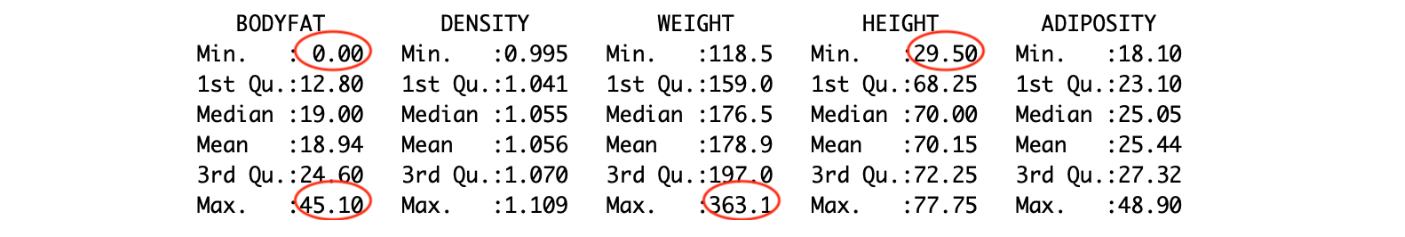
\includegraphics{plots/summary.png}

The observations that have extreme values are

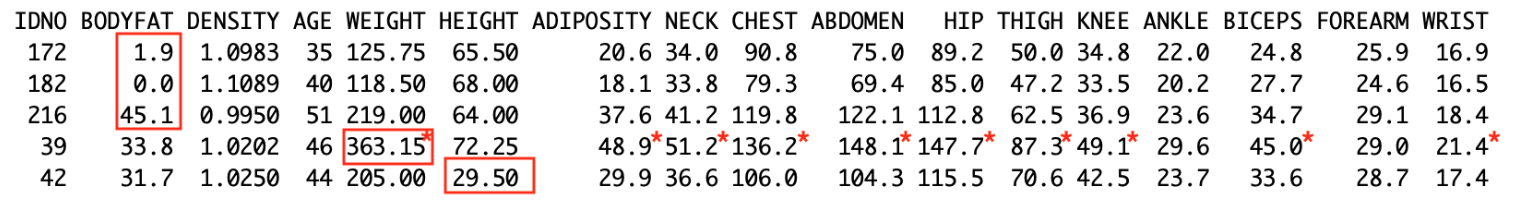
\includegraphics{plots/data1.png}

    \textbf{BODYFAT} is the response variable whose reasonable value ranges
from 2\% to 39\%. Individual 172 has lowest possible body fat, which can
be considered as essential fat; Individual 216 is sever obesity, which
is possible; Individual 182, it's impossible to have 0\% of bodyfat, and
after checking the siri's equation to his density, the corresponding
bodyfat becomes negative, thus we filter this records out of our
analysis.

There also exists extreme value in \textbf{WEIGHT}, which occurs in
individual 39. This man also has the largest value in ADIPOSITY, NECK,
CHEST, ABDOMEN, HIP, THIGH, KNEE, BICEPS, and WRIST. Which indicates
that this record does exist.

As for \textbf{HEIGHT}, individual 42's height is only 29.5 which is
quite abnormal. After checking the corresponding weight by BMI formula,
we can assume that this is a wrong record. Thus we fix his height by
applying the BMI formula.

    \hypertarget{check-siris-equation}{%
\subsection{Check Siri's Equation}\label{check-siris-equation}}

Known that the body fat percentage can be estimated by the density with
the Siri's equation. We build a linear model between the bodyfat
percentage estimated by Siri's equation and the bodyfat percentage in
the data set. The residual plot and the QQ plot of this model is shown
below. We can see that record 48, 76, 96 are possible outliers.


\includegraphics{plots/data2_1.png}

    Individual 96's other variables all have normal value, which indicates
his desity might be wrongly recorded.

Individual 48 and 76 have similar values in other variables, thus their
body fat percentage should also be similar. Thus we use the Siri's
equation to fix their body fat percentage.

    \hypertarget{check-the-bmi-formula}{%
\subsection{Check the BMI Formula}\label{check-the-bmi-formula}}

Known that the ADIPOSITY can be estimated using WEIGHT and HEIGHT. We
build a linear model between the BMI estimated by equation and the
ADIPOSITY in the data set. The residual plot and the QQ plot of this
model is shown below. We can see that record 163, 220, 234 are possible
outliers.

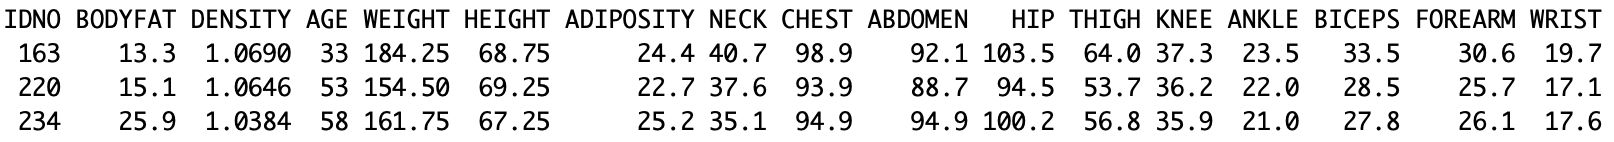
\includegraphics{plots/data3_1.png}

    For individual 163, 220, and 234, their weights vary a lot, which means
their BMI should not be similar to each other. Thus we adopt the
calculated BMI as their ADIPOSITY.

    \hypertarget{data-cleaning-summary}{%
\subsection{Data cleaning summary}\label{data-cleaning-summary}}

In conclusion:

Record \textbf{182} is filtered out because it has 0 body fat and
there's no way to fix that.

The HEIGHT of record \textbf{42} is fixed according to the weight and
adiposity.

The body fat of record \textbf{48} and \textbf{76} are fixed according
to the density.

The adiposity of record \textbf{163}, \textbf{220}, and \textbf{234} are
fixed according to the weight and height.

    \hypertarget{variable-selection-and-statistical-modeling}{%
\section{Variable Selection and Statistical
Modeling}\label{variable-selection-and-statistical-modeling}}

\hypertarget{variable-selection}{%
\subsection{Variable Selection}\label{variable-selection}}

\hypertarget{stepwise-backward-and-forward-lr}{%
\subsubsection{Stepwise Backward and Forward
LR}\label{stepwise-backward-and-forward-lr}}

Considering there is a tradeoff between model variance and accuracy,
we'd better not use all 14 predictors to establish the model. Although
the mean square of error (MSE) will be small, the model itself will be
unstable. Firstly, we try normal linear regression using the stepwise
method to select features. We chose BIC as criterion and directions of
forward and backward. The result was shown respectively.

    A matrix: 5 × 4 of type dbl
\begin{tabular}{r|llll}
  & Estimate & Std. Error & t value & Pr(>\textbar{}t\textbar{})\\
\hline
	(Intercept) & -29.9234561 & 6.69406028 & -4.470150 & 1.193678e-05\\
	ABDOMEN &   0.9133283 & 0.05163326 & 17.688759 & 9.869649e-46\\
	WEIGHT &  -0.1238172 & 0.02276101 & -5.439883 & 1.285958e-07\\
	WRIST &  -1.4082304 & 0.40713801 & -3.458853 & 6.391933e-04\\
	FOREARM &   0.4253252 & 0.16733889 &  2.541700 & 1.164621e-02\\
\end{tabular}


    
    The results of backward and forward method are the same, WEIGHT,
ABDOMEN, FOREARM, WRIST were chosen as predictors and they are all
significant. R-square of the model is 0.736, which indicates the
accuracy of the model is quite good. However, in the linear model,
collinearity of predictors will increase the variance of model. VIF is a
value to identify collinearity. There are collineary between variables
if VIF is larger than 5.

    \begin{Verbatim}[commandchars=\\\{\}]
 ABDOMEN   WEIGHT    WRIST  FOREARM 
4.789592 6.924539 2.242982 1.770719 

    \end{Verbatim}

    The model is still unstable, so we try other methods to do variable
selection.

    \hypertarget{variable-selection-with-xgboost}{%
\subsubsection{Variable Selection with
XGBoost}\label{variable-selection-with-xgboost}}

XGBoost is an ensemble learning method with tree models. It will output
the importance of variables after establishing the model. The criterion
for ranking predictors is how many times the variable is chosen as the
node in decision trees. The more frequent it is chosen the larger score
it will get. Moreover, if the variable is chosen near root of tree, the
score will has a large weight because its influence to the decision tree
is large.

    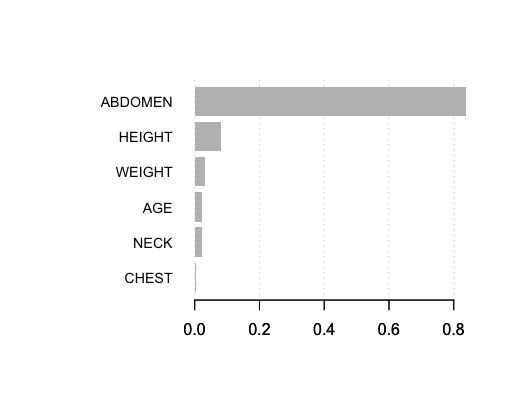
\includegraphics{plots/xgboost.png}

    \hypertarget{stable-statistical-model}{%
\subsection{Stable Statistical Model}\label{stable-statistical-model}}

In both of our methods, we find that ABDOMEN is the most important
variable among 14 predictors. WEIGHT ranks high in both methods
comparing with other variables. WRIST is significant in linear stepwise
model and ADIPOSITY scores high in nonlinear model. Considering the rule
of thumb, we select ABDOMEN as our first variable in predicting body
fat. Also, to increase the accuracy we choose another variable among
WRIST, WEIGHT, ADIPOSITY as our second variable. The number of
predictors are too small to use any tree model or ensemble method in
machine learning. We still choose normal linear regression as our model.
The collinearity are not significant between two variables, so we may
not add regulization to our model. After comparing three models, we
choose ABDOMEN and WEIGHT as our predictors, because it has highest
R-square 0.72.

    A matrix: 3 × 4 of type dbl
\begin{tabular}{r|llll}
  & Estimate & Std. Error & t value & Pr(>\textbar{}t\textbar{})\\
\hline
	(Intercept) & -40.6768857 & 2.41526710 & -16.841568 & 5.953549e-43\\
	ABDOMEN &   0.9082391 & 0.05222159 &  17.392023 & 7.810903e-45\\
	WEIGHT &  -0.1364208 & 0.01914546 &  -7.125489 & 1.124027e-11\\
\end{tabular}


    
    \hypertarget{model-diagnostics-strength-and-weekness}{%
\subsection{Model Diagnostics \& Strength and
Weekness}\label{model-diagnostics-strength-and-weekness}}

\hypertarget{final-model}{%
\subsubsection{Final Model:}\label{final-model}}

\[BODYFAT (\%) = 0.908*ABDOMEN(cm) - 0.136*WEIGHT(lb)\] \#\#\# Model
Diagnostics:

Firstly, use VIF to check collinearity. There is no obvious collinearity
between ABDOMEN and WEIGHT.

    print(vif(fit1))

    Then, plot the residuals vs fitted values. Residuals are seperated
randomly near 0 and there is no correlation between fitted value and
residuals. Also, there is no correlation between residuals and
predictors. QQ-plot of residuals show that residuals generally follows
normal distribution. It is normal that there are still some outliers in
the model.

    \begin{center}
    \adjustimage{max size={0.9\linewidth}{0.9\paperheight}}{STAT628_Module_2_Group_9_files/STAT628_Module_2_Group_9_23_0.png}
    \end{center}
    { \hspace*{\fill} \\}
    
    \hypertarget{strength-and-weakness-of-our-model}{%
\subsubsection{Strength and Weakness of our
model:}\label{strength-and-weakness-of-our-model}}

Generally, this model is a simple, robust, accurate and efficient model.
It satisfies assumptions in linear regression model and explains 72\% of
the variation in body fat \% among men although. It also has weaknesses
as it cannot capture higher order effects and interactions.

\hypertarget{shiny-app}{%
\section{Shiny APP}\label{shiny-app}}

Based on the model above, we developed the shiny app.

\hypertarget{extra-packages}{%
\paragraph{Extra packages}\label{extra-packages}}

Beside the ``shiny'' package, we also used ``shinybulma'', ``grid'',
``png'', ``bs4Dash'', ``rsconnect'', ``ggplot2'', ``shinyalert''.

\hypertarget{function}{%
\paragraph{Function}\label{function}}

\begin{enumerate}
\def\labelenumi{\arabic{enumi}.}
\tightlist
\item
  Body Fat calculator
\item
  Size converter(kg to lbs, inch to cm)
\item
  Detail information about body fat
\end{enumerate}

\hypertarget{web-based-app-link}{%
\paragraph{Web-based app Link}\label{web-based-app-link}}

https://jiawen1014.shinyapps.io/BodyFat/

\hypertarget{contribution}{%
\section{Contribution}\label{contribution}}

Jiawen Chen: Web-based App\\
Chunyuan Jin: Model building and model diagnosing\\
Han Liao: Data cleaning


    % Add a bibliography block to the postdoc
    
    
    
    \end{document}
